\documentclass[aspectratio=169]{beamer}
\usetheme{Madrid}
\usepackage{amsmath, amssymb}
\usepackage{graphicx}
\usepackage{tikz}

\title{Progress Report}
\subtitle{Objective of Score matching on non-negative data}
\author{Kamiya Takuto}
\date{\today}
\begin{document}
\begin{frame}
  \titlepage
\end{frame}
\begin{frame}{Outline}

\begin{itemize}
  \item \textcolor{black}{1. Review of Score Matching}
  \vspace{0.5em}
  \item \textcolor{black}{2. Score Matching on Non-negative Data}
  \begin{itemize}
    \item \textcolor{black}{(1) Weighted Score Matching}
    \item \textcolor{black}{(2) Proposed Method: Boundary Term Approximation}
  \end{itemize}
\end{itemize}

\end{frame}

\begin{frame}{Score Function}
\begin{block}{Score Function}
\[
\nabla_x \log p(x) = \left(
\frac{\partial}{\partial x_1}\log p(x), \dots,
\frac{\partial}{\partial x_m}\log p(x)
\right)^\top \left(\space x\in \mathbb{R}^m\right)  
\]
\end{block}
\vspace{0.5em}
\textbf{Key property:} The score function is \emph{invariant under normalization}.

\vspace{0.5em}
Let \( p(x) = \frac{\tilde{p}(x)}{Z} \), where \( Z = \int \tilde{p}(x) dx \) is the partition function. Then:
$$
\nabla_x \log p(x) = \nabla_x \log \tilde{p}(x)\quad \text{since } \log p(x) = \log \tilde{p}(x) - \log Z
$$

\vspace{0.5em}
The normalization constant \( Z \) disappears under differentiation.

\end{frame}
\begin{frame}{Objective of Score Matching}

\begin{block}{Score Matching Loss}
$$
 J(p) = \int_{\mathbb{R}^m}\|\nabla_x \log p(x) - \nabla_x\log q(x)\|^2 q(x)dx
$$
\end{block}

\vspace{1em}
This loss measures the discrepancy between the score functions of the model \( p \) and the data distribution \( q \), 
using an expectation under  \( q(x) \).

\[
\hat{\theta} = \operatorname*{argmin}_{\theta} J(p_{\theta}, q) 
= \operatorname*{argmin}_{\theta}\int_{\mathbb{R}^m}
\|\nabla_x \log p_\theta(x) - \nabla_x\log q(x)\|^2 q(x)dx
\]

\vspace{1em}
We estimate the model parameter \( \theta \) by minimizing the score-matching objective.

\end{frame}
\begin{frame}{Approach to Reformulating the Objective}
    We begin by expressing the score matching loss as:

\[
J = \int_{\mathbb{R}^m} F(x) \, q(x) \, dx \quad \Longleftrightarrow \quad J = \mathbb{E}_{x \sim q}[F(x)]
\]

\vspace{1em}

This suggests we can approximate \( J \) using the empirical average:

\[
\mathbb{E}_{x \sim q}[F(x)] \approx \frac{1}{n} \sum_{i=1}^n F(x_i)
\]

\vspace{1em}

However, in its current form, \( F(x) \) still depends on \( q(x) \), which is unknown.

\textbf{Goal:} Reformulate the objective so that
\[
J = \int_{\mathbb{R}^m} F'(x) \, q(x) \, dx
\]
where \( F'(x) \) no longer involves \( q(x) \). This enables unbiased empirical estimation.
\end{frame}
\begin{frame}{Fisher Divergence as a Decomposed Divergence}

\begin{itemize}
  \item Expanding the squared norm in $J(p)$ gives:
  \[
\int \|\nabla_x \log p(x)\|^2 \, q(x) \, dx
  - 2 \int \nabla_x \log p(x)^\top \nabla_x \log q(x)\, q(x) \, dx
  + \int \|\nabla_x \log q(x)\|^2 \, q(x) \, dx
  \]
  \item This can be written in the form:
  \[
 J(p) = g(q) + d(p, q)
  \]
  where
  \[
  g(q) = \int \|\nabla_x \log q(x)\|^2 \, q(x) \, dx,
  \]
  \[
  d(p, q) = \int \|\nabla_x \log p(x)\|^2 \, q(x) \, dx
  - 2 \int \nabla_x \log p(x)^\top \nabla_x \log q(x) \, q(x) \, dx
  \]

\end{itemize}
\end{frame}
\begin{frame}{Structure of \( J(p) = d(p, q) \)}

Since \( g(q) \) does not depend on the model \( p \), minimizing \( J(p) \) is equivalent to minimizing \( d(p, q) \).  
  \textbf{Thus, we redefine \( J(p) := d(p, q) \) for the remainder of this presentation.}:
\[
J(p) = \int \|\nabla_x \log p(x)\|^2 \, q(x) \, dx
- 2 \int \nabla_x \log p(x)^\top \nabla_x \log q(x) \, q(x) \, dx
\]

\vspace{1em}
This objective consists of two terms:
\begin{itemize}
  \item The first term depends only on the model \( p \), via its score function.
  \item The second term couples the model score \( \nabla_x \log p(x) \) with the data score \( \nabla_x \log q(x) \), and is problematic because \( \nabla_x \log q(x) \) is unknown.
\end{itemize}

\vspace{1em}
\textbf{Goal:} Eliminate the dependence on the unknown \( \nabla_x \log q(x) \) using integration by parts.
\end{frame}
\begin{frame}{Step 1: Substituting the Score Function}

We begin with the problematic term:
\[
-2 \int \nabla_x \log p(x)^\top \nabla_x \log q(x) \, q(x) \, dx.
\]

Using the identity:
\[
\nabla_x \log p(x) = \frac{\nabla_x q(x)}{q(x)}
\quad \Rightarrow \quad
\nabla_x \log q(x) \cdot q(x) = \nabla_x q(x),
\]
we rewrite:
\[
-2 \int \nabla_x \log p(x)^\top \nabla_x \log q(x) \, q(x) \, dx
= -2 \int  \nabla_x \log p(x)^\top \nabla_x q(x)\, dx.
\]

\vspace{1em}
\textbf{This step assumes:}
\begin{itemize}
  \item \( q(x) > 0 \) almost everywhere,
  \item \( q \in C^1(\mathbb{R}^d) \),
  \item The integral is well-defined and finite.
\end{itemize}
\end{frame}
\begin{frame}{Step 2: Integration by Parts}
We now handle the term:
\[
-2 \int \nabla_x \log p(x)^\top \nabla_x q(x) \, dx.
\]

Component-wise:
\[
= -2 \sum_{i=1}^m \int   \frac{\partial}{\partial x_i} \log p(x) \cdot\frac{\partial q(x)}{\partial x_i}\, dx.
\]

By integration by parts:
\[
= 2 \sum_{i=1}^m \int\frac{\partial^2}{\partial x_i^2} \log p(x) \cdot q(x)\, dx
= 2 \int  \Delta_x \log p(x) \cdot p(x)\, dx.
\]

\textbf{Assumption:} boundary term vanishes,
\[
\lim_{\|x\| \to \infty} \frac{\partial}{\partial x_i} \log p(x) \cdot q(x)= 0.
\]
\end{frame}
\begin{frame}{Final Form of \( J(p) \)}
Combining the two terms, we have:
\[
J(p)
= \int \|\nabla_x \log p(x)\|^2 \, q(x)\, dx
+ 2 \int \Delta_x \log p(x)\, q(x)\, dx.
\]

\textbf{Key features:}
\begin{itemize}
  \item The expression depends only on the model \( p \),
  \item The expectation is taken under \( q(x) \), which can be approximated from data.
\end{itemize}

This forms the basis of the score matching objective.
\end{frame}
\begin{frame}{Empirical Score Matching Objective}
From the previous analysis, we obtained the following quantity to minimize:
\[
J(p) = \int \left( \|\nabla_x \log p(x)\|^2 + 2 \Delta_x \log p(x) \right) q(x)\, dx.
\]

This is an expectation over the data distribution \( p(x) \), which is unknown.\\[1ex]

However, given i.i.d. samples \( x^{(1)}, \dots, x^{(n)} \sim p(x) \), we approximate it as:
\[
\hat{J}(p) = \frac{1}{n} \sum_{i=1}^n \left( \|\nabla_x \log p(x^{(i)})\|^2 + 2 \Delta_x \log p(x^{(i)}) \right).
\]



\end{frame}
\begin{frame}{Outline}

\begin{itemize}
  \item \textcolor{gray}{1. Review of Score Matching}
  \vspace{0.5em}
  \item \textcolor{black}{2. Score Matching on Non-negative Data}
  \begin{itemize}
    \item \textcolor{black}{(1) Weighted Score Matching}
    \item \textcolor{gray}{(2) Proposed Method: Boundary Term Approximation}
  \end{itemize}
\end{itemize}

\end{frame}
\begin{frame}{Score Matching for Non-negative Data}
\begin{block}{Weighted Score Matching}
Let \( h_1, \ldots, h_m : \mathbb{R}_+ \to \mathbb{R}_+ \) be a.s.\ positive functions that are absolutely continuous on every bounded subinterval of \( \mathbb{R}_+ \), and set
$
h(x) = \left[h_1(x_1), \ldots, h_m(x_m)\right]^\top,
$
which is absolutely continuous on \( \mathbb{R}_+^m \).\\
\vspace{5mm}
Then, the weighted score matching objective is defined as
\[
J_h(p) = \int_{\mathbb{R}_+^m} \left\| h(x)^{1/2} \odot \nabla_x \log p(x) - h(x)^{1/2} \odot \nabla_x \log q(x) \right\|^2 q(x)\, dx, 
\]
where
$
h(x) ^{1/2} = \left[h_1(x_1)^{1/2} , \ldots, h_m(x_m)^{1/2} \right]^\top,
$
and $\odot$ is denote the element-wise product 
$$\Big(\mathbf{y} \odot \mathbf{z} = [y_1 \cdot z_1, \cdots, y_m \cdot z_m] \ \ \  \mathbf{y},\mathbf{z} \in \mathbb{R}^m\Big)$$
\end{block}
\end{frame}
\begin{frame}{Rewriting Weighted Score Matching Objective}

We expand the weighted score matching loss:

\[
J_h(p) = \int_{\mathbb{R}_+^m} \left\| h(x)^{1/2} \odot \left(\nabla_x \log p(x) - \nabla_x \log q(x)\right) \right\|^2 q(x)\, dx - C(q)=
\]

\[
\int_{\mathbb{R}_+^m} \left\| h(x)^{1/2} \odot \nabla_x \log p(x) \right\|^2 q(x)\, dx
- 2 \int_{\mathbb{R}_+^m} \left( h(x) \odot \nabla_x \log p(x) \right)^\top
\left( h(x) \odot \nabla_x \log q(x) \right) q(x)\, dx
+ C(q)
\]

where \( C(q) = \int \left\| h(x)^{1/2} \odot \nabla_x \log q(x) \right\|^2 q(x) dx \) is constant in \( p \).

\vspace{1em}
\textbf{Goal:} Eliminate dependence on \( \nabla_x \log q(x) \) via integration by parts.

\end{frame}
\begin{frame}{Integration by Parts with Weight Function}

We now handle the cross term:

\[
\int_{\mathbb{R}_+^m} 
\left( h(x)^{1/2} \odot \nabla_x \log p(x) \right)^\top 
\left( h(x)^{1/2} \odot \nabla_x \log q(x) \right) q(x)\, dx
\]

\[
= \int_{\mathbb{R}_+^m} 
\left( h(x) \odot \nabla_x \log p(x) \right)^\top 
\nabla_x \log q(x) \cdot q(x)\, dx
= \int \left( h(x) \odot \nabla_x \log p(x) \right)^\top \nabla_x q(x)\, dx
\]

\vspace{1em}
Then, by component-wise integration by parts:
\[
= - \int \operatorname{div}(h(x) \odot \nabla_x \log p(x)) \cdot q(x)\, dx + \text{boundary term}
\]

\textbf{Assumption:} boundary term vanishes or is handled separately.

\end{frame}
\begin{frame}{Final Objective: Weighted Score Matching}

Combining all terms, we get:

\[
J_h(p) = \int_{\mathbb{R}_+^m} \left(
\left\| h(x)^{1/2} \odot \nabla_x \log p(x) \right\|^2 
+ 2 \cdot \operatorname{div}(h(x) \odot \nabla_x \log p(x)) 
\right) q(x)\, dx
\]

\vspace{1em}
\textbf{Empirical Approximation:}  
Given samples \( x^{(1)}, \dots, x^{(n)} \sim q(x) \), we approximate \( J_h(p) \) by:

\[
\hat{J}_h(p) = \frac{1}{n} \sum_{i=1}^n \left(
\left\| h(x^{(i)})^{1/2} \odot \nabla_x \log p(x^{(i)}) \right\|^2 
+ 2 \cdot \operatorname{div}(h(x^{(i)}) \odot \nabla_x \log p(x^{(i)})) 
\right)
\]

\end{frame}
\begin{frame}{Outline}

\begin{itemize}
  \item \textcolor{gray}{1. Review of Score Matching}
  \vspace{0.5em}
  \item \textcolor{black}{2. Score Matching on Non-negative Data}
  \begin{itemize}
    \item \textcolor{gray}{(1) Weighted Score Matching}
    \item \textcolor{black}{(2) Proposed Method: Boundary Term Approximation}
  \end{itemize}
\end{itemize}

\end{frame}

\begin{frame}{Proposed Method: Score Matching on Domain \( M \)}

We propose a modified score matching objective over a domain \( M \subset \mathbb{R}^m \) with boundary \( \partial M \).

\vspace{1em}
\begin{block}{Proposed objective}
\[
J_{\text{prop}}(p) = \int_M \|\nabla \log p(x)\|^2 q(x)\, dx
+ 2 \int_M \Delta \log p(x) \cdot q(x)\, dx
+ 2 B(p, q)
\]
\end{block}
where \( B(p, q) \) denotes the \textbf{boundary term} arising from applying Stokes' theorem to the cross term.

\vspace{1em}

\textbf{Key difference from conventional score matching:}  
The boundary term \( B(p, q) \) is preserved rather than discarded.

\end{frame}
\begin{frame}{Boundary Term in the Proposed Objective}

The boundary term \( B(p, q) \) has the following explicit form:

\[
B(p, q) = - \int_{\partial M} \left( \nabla \log p(x) \cdot \mathbf{n}(x) \right) q(x)\, dS(x)
\]

\vspace{1em}

\textbf{Explanation:}
\begin{itemize}
  \item \( \mathbf{n}(x) \): outward unit normal vector on the boundary \( \partial M \),
  \item \( dS(x) \): surface measure on \( \partial M \),
\end{itemize}

\vspace{1em}

\textbf{Interpretation:}  
It penalizes mismatch between the model flow and the data density near the boundary.

\end{frame}
\begin{frame}{Case \( M = \mathbb{R}^m_+ \)}
\begin{columns}
  % 左カラム:数式
  \begin{column}{0.55\textwidth}
    \begin{flushleft}
    For simplicity, let us assume:
    \[
    M = \mathbb{R}_+^m = \{(x_1, \cdots,x_m) \mid x_1, \cdots,x_m \geq 0\}
    \]
    \[
    H_i = \{(x_1,  \cdots,x_m) \in \mathbb{R}_+^m \mid x_i = 0\}
    \]
    Then, the each component is 
    \[
    \partial M = \sum_{i=1}^{m} H_i
    \]
    \[
    \mathbf{n}(x) = -e_i \quad (x \in H_i)
    \]
    \[
    dS(x) = dx_{-i} = dx_1 \dots dx_{i-1} dx_{i+1} \dots dx_m \quad (x \in H_i)
    \]
    \end{flushleft}
  \end{column}

  % 右カラム:図(例としてimage.pngを挿入)
  \begin{column}{0.45\textwidth}
    \begin{center}
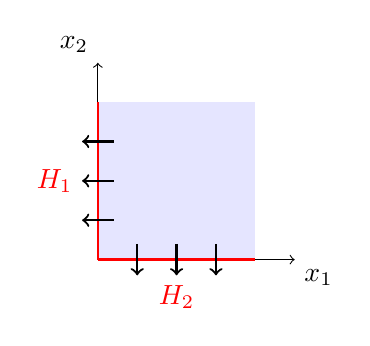
\begin{tikzpicture}
  % 座標軸
  \draw[->] (0,0) -- (2.5,0) node[below right] {$x_1$};
  \draw[->] (0,0) -- (0,2.5) node[above left] {$x_2$};

  % 域 M
  \fill[blue!10] (0,0) -- (2,0) -- (2,2) -- (0,2) -- cycle;

  % 境界 H1
  \draw[thick, red] (0,0) -- (0,2);
  \node[red, left] at (-0.2,1) {$H_1$};

  % 境界 H2
  \draw[thick, red] (0,0) -- (2,0);
  \node[red, below] at (1,-0.2) {$H_2$};

  % 法線ベクトル on H1
  \draw[->, thick] (0.2,1.5) -- (-0.2,1.5);
  \draw[->, thick] (0.2,1) -- (-0.2,1);
  \draw[->, thick] (0.2,0.5) -- (-0.2,0.5);

  % 法線ベクトル on H2
  \draw[->, thick] (1.5,0.2) -- (1.5,-0.2);
  \draw[->, thick] (1,0.2) -- (1,-0.2);
  \draw[->, thick] (0.5,0.2) -- (0.5,-0.2);
\end{tikzpicture}
    \end{center}
  \end{column}
\end{columns}
\end{frame}
\begin{frame}{Transforming \( B(p,q) \) and Preparing for Empirical Estimation}

We start from the boundary term:
\[
B(p, q) = - \int_{\partial M} \left( \nabla \log p(x) \cdot \mathbf{n}(x) \right) q(x)\, dS(x)
\]

In the case \( M = \mathbb{R}_+^m \), this becomes:
\[
= \sum_{i = 1}^m \int_{H_i} \frac{\partial}{\partial x_i} \log p(x) \cdot q(x_i = 0, x_{-i}) \, dx_{-i}
\]

To make empirical estimation feasible, we rewrite the joint density using the identity:
\[
q(x_i = 0, x_{-i}) = q(x_i = 0) \cdot q(x_{-i} \mid x_i = 0)
\]

Hence:
\[
= \sum_{i = 1}^m q(x_i = 0) \int_{H_i} \frac{\partial}{\partial x_i} \log p(x) \cdot q(x_{-i} \mid x_i = 0) \, dx_{-i}
\]



\end{frame}
\begin{frame}{Empirical Approximation of the Boundary Term}

We consider the following form of the boundary term:
\[
B(p, q) = \sum_{i=1}^m q(x_i = 0) \cdot \mathbb{E}_{x_{-i} \sim q(x_{-i} \mid x_i = 0)}
\left[ \frac{\partial}{\partial x_i} \log p(x_i=0, x_{-i}) \right]
\]

Since exact sampling from \( x_i = 0 \) is infeasible, we approximate using small \( \epsilon > 0 \):

\vspace{1em}

\textbf{Density at the boundary:}
\[
q(x_i = 0) = \lim_{\epsilon \rightarrow 0} \frac{\mathbb{P}(0 \leq x_i < \epsilon)}{\big|\{0 \leq x_i < \epsilon\}\big|}  
\approx \frac{n_i^\epsilon}{n \epsilon}
\quad \Big(n_i^\epsilon = \sum_{j = 1}^n \mathbf{1}_{\{x|0 \leq x_i < \epsilon\}}(x^{(j)})\Big)
\]

\textbf{Conditional expectation:}
\[
\mathbb{E}_{x_{-i} \sim q(x_{-i} \mid x_i = 0)} \left[ \frac{\partial}{\partial x_i} \log p(x) \right]
\approx \frac{1}{n_i^\epsilon} \sum_{j=1}^n 
\frac{\partial}{\partial x_i} \log p(x^{(j)})\mathbf{1}_{\{x|0 \leq x_i < \epsilon\}}(x^{(j)})
\]

\end{frame}
\begin{frame}{Final Empirical Objective with Boundary Term}

\textbf{Final approximation of \( B(p, q) \):}
\[
\hat{B}(p, q) 
= \frac{1}{n \epsilon} \sum_{i=1}^m \sum_{j=1}^n 
\frac{\partial}{\partial x_i} \log p(x^{(j)}) 
\cdot \mathbf{1}_{\{0 \leq x_i^{(j)} < \epsilon\}}(x^{(j)})
\]

\vspace{1em}

\textbf{Thus, the full empirical objective becomes:}
\[
\hat{J}(p) 
= \frac{1}{n} \sum_{j=1}^n \sum_{i=1}^m 
\left( \frac{\partial}{\partial x_i} \log p(x^{(j)}) \right)^2
+ 2 \cdot \frac{\partial^2}{\partial x_i^2} \log p(x^{(j)})
+ \frac{2}{\epsilon} \cdot \frac{\partial}{\partial x_i} \log p(x^{(j)}) 
\cdot \mathbf{1}_{\{0 \leq x_i^{(j)} < \epsilon\}}(x^{(j)})
\]

\vspace{0.5em}
\textbf{where } \( x^{(j)} \sim q(x) \), and \( \epsilon > 0 \) controls boundary proximity.

\end{frame}
\begin{frame}{Experimental Comparison: Weighted  vs. Proposed Score Matching}
\begin{columns}
  % 左:指数分布
  \begin{column}{0.48\textwidth}
    \centering
    \textbf{Exponential Distribution} \\[0.5em]
    \includegraphics[width=\linewidth]{exp_result.png} \\[0.5em]

    \textbf{Estimated Parameters:}
    \begin{itemize}
      \item Weighted: \quad \( \hat{\theta}_w = 2\bar{x}/\bar{x^2}  \)
      \item Proposed: \quad \( \hat{\theta}_p = |H_i^\epsilon|/n\epsilon \)
    \end{itemize}
  \end{column}

  % 右:切断正規分布
  \begin{column}{0.48\textwidth}
    \centering
    \textbf{Truncated Normal Distribution} \\[0.5em]
    \includegraphics[width=\linewidth]{truncnorm_result.png} \\[0.5em]

    \textbf{Estimated Parameters:}
    \begin{itemize}
      \item Weighted: \quad \( \hat{\theta_i}_w = \bar{x_i^4}/3\bar{x_i^2} \)
      \item Proposed: \quad \( \hat{\theta}_p = n\epsilon\bar{x_i^2}/\left(\sum x_i^\epsilon + n\epsilon\right)\)
    \end{itemize}
  \end{column}
\end{columns}

\vspace{1em}
\textbf{Observation:} The proposed method produces more accurate estimates near the boundary, particularly for non-smooth densities.

\end{frame}
\begin{frame}{References}

\small

\begin{thebibliography}{99}

\bibitem{Yu2021}
Yu, S., Drton, M., \& Shojaie, A. (2021). 
\newblock Generalized Score Matching for General Domains.
\newblock {\em Information and Inference: A Journal of the IMA}, 11(2), 739--780.
\newblock \url{https://doi.org/10.1093/imaiai/iaaa041}

\end{thebibliography}

\end{frame}

\end{document}